%%%%%%%%%%%%%%%%%%%%%%%%%%%%%%%%%%%%%%%%%%%%%%%%%%%%%%%%%%%%%%%
% P3b MLP
% David Miguel Lozano
% Javier Martínez Riberas
% Universidad de Burgos - Noviembre 2016
%%%%%%%%%%%%%%%%%%%%%%%%%%%%%%%%%%%%%%%%%%%%%%%%%%%%%%%%%%%%%%%

% -------------------------------------------------------------
% Preamble
% -------------------------------------------------------------
\documentclass[a4paper,12pt,titlepage]{article}

% -------------------------------------------------------------
% Packages
% -------------------------------------------------------------
\usepackage[utf8]{inputenc}	% Unicode support
\usepackage[T1]{fontenc}		% Font encoding
\usepackage[spanish]{babel}	% Languaje
\usepackage{lmodern}	% Typeface 
\usepackage{textcomp} % Special symbols
\usepackage{graphicx}	% Add pictures
\usepackage{pgfplots} % Graphs and charts
\usepackage{hyperref}	% Add a link to index entries
\usepackage{amsmath}	% Advanced math typesetting
\usepackage{amsfonts}	% Mathematical formulas
\usepackage{amssymb}	% Extended symbol collection
\usepackage{listings}	% Code formatting and highlighting
\usepackage{xcolor}		% Color package
\usepackage{enumitem}	% Customizing lists
\usepackage{parskip}	% Paragraph styles
\usepackage[a4paper]{geometry} 		% Margins
\usepackage[numbers,sort]{natbib}	% Bibliography management
\usepackage{booktabs}							% Tables

% -------------------------------------------------------------
% Configuration
% -------------------------------------------------------------
% Images path
\graphicspath{ {img/} }
% Graphs configuration 
\pgfplotsset{width=\textwidth,compat=1.9}
% Hyperlinks coloring
\hypersetup{
	colorlinks,
	linkcolor={green!40!black},
	citecolor={blue!50!black},
	urlcolor={blue!80!black}
}
% Define HRule
\newcommand{\HRule}[1]{\rule{\linewidth}{#1}}
% Define listings styles
\definecolor{codebg}{HTML}{EEEEEE}
\definecolor{codeframe}{HTML}{CCCCCC}
\definecolor{comments}{HTML}{009900}
\lstset{
  language=Matlab, 								% Programming language 
  backgroundcolor=\color{codebg},	% Background color
  frame=single, 									% Add frame around code
	framesep=10pt,									% Padding
	rulecolor=\color{codeframe},		% Don't change frame color
	upquote=true,										%
	breakatwhitespace=true,					% Break line only in spaces
	keepspaces=true,								% Keep indentation
	tabsize=2,											% Tab size
	title=\lstname, 								% Show filename as caption
	basicstyle=\ttfamily, 					% Size and font
  keywordstyle=\color{black}\ttfamily,
	commentstyle=\color{comments},	% Color of comments
  morecomment=[l][\color{magenta}]{\#}
}
% Define style table
\setlength{\heavyrulewidth}{1.5pt}
\setlength{\abovetopsep}{4pt}
\begin{document}
% -------------------------------------------------------------
% Cover
% -------------------------------------------------------------
\author{David Miguel Lozano \ Javier Martínez Riberas}
\title{P3 Multilayer Perceptron (MLP)}
\date{07-11-2016}

\begin{titlepage}
	\centering
	
\includegraphics[width=0.16\textwidth]{ubu-logo.png}\par
	\vspace{0.3cm}
	{\scshape\LARGE Universidad de Burgos \par}
	\vfill
	{\scshape\Large Computación Neuronal y Evolutiva \par}
	\HRule{2pt}
	{\huge\bfseries P4: AirTafficController \par}
	\HRule{2pt}
	\\ [0.5cm]
	{Analizar y desarrollar un algoritmo genético que realice el cálculo automático de la distribución más conveniente de vuelos que solicitan aterrizar en un determinado aeropuerto.}
	\vfill
	Estudiantes:\par
	{\Large\scshape David Miguel Lozano \\ Javier Martínez Riberas \par}
	\vfill
	Profesor de la asignatura:\par
	\textsc{Bruno Baruque Zanón}
	\vfill
	{\large 1º semestre 2016 \par}
\end{titlepage}

% -------------------------------------------------------------
% Contents
% -------------------------------------------------------------
\newpage
\tableofcontents
\begin{appendix}
  %\listoffigures
  %\listoftables
\end{appendix}

% -------------------------------------------------------------
% Body
% -------------------------------------------------------------
\newpage

\section{Introducción}

El objetivo de esta práctica es desarollar un programa que implemente un algoritmo genético que permita al usuario realizar el calculo automático de la distribución
más conveniente de vuelos que solicitan aterrizar en un determinado aeropuerto. Así mismo, se analizará la conveniencia de la solución propuesta y se reflexionará sobre los resultados obtenidos.

La aplicación tiene que ser capáz de adaptarse a las siguientes condiciones:

\begin{itemize}[noitemsep]
	\item El número de pistas del aeropuerto debe ser un parámetro configurable.
	\item El número de aviones en cada situación puede variar.
	\item Los aviones tienen un programa de vuelo que incluye:
	\begin{itemize}[noitemsep]
		\item ETA (\textit{Estimated Time of Arrival}): tiempo estimado de llegada calculado en el momento del despegue.
		\item Tipo de avión: heavy / big / small. Condiciona el tiempo necesario para su aterrizaje.
	\end{itemize}
\end{itemize}

El programa tiene que conseguir obtener de forma automática la mejor asignación posible de vuelos a aterrizar en cada pista, de forma que el tiempo de espera de los vuelos en su conjunto sea el menor posible.

Para su resolución se hará uso de la librería para Java JCLEC (Java Class Library for Evolutionary Computation) \citep{web:jclec}. La cual, proporciona un framework para programación evolutiva que da soporte, entre otras cosas, a los algoritmos genéticos.

\section{Solución propuesta}

A continuación se detalla la codificación y configuración del problema para ser resuelto con un algoritmo genético.

\subsection{Representación de los individuos}

Para representar los individuos se ha utilizado un array de enteros ordenado (\lstinline|OrderArrayIndividual|). Se probaron dos representaciones diferentes, en ambas cada posición del array representaba un avión, pero el ordenamiento era distinto:

\begin{enumerate}[noitemsep]
	\item Array ordenado por orden de llegada. De tal manera, que la primera posición se correspondía con el primer avión en llegar. Y el valor de cada posición indicaba el número del avión.
	\item Array ordenado por número de avión. De tal manera, que la primera posición se correspondía con el avión número uno. Y el valor de cada posición indicaba la posición de llegada del avión.
\end{enumerate}

Tras realizar pruebas, se vió que los resultados eran muy similares. Por lo que se eligió la representación 1 para realizar el estudio.

Ejemplo de genotipo:

\begin{center}
$
\begin{bmatrix}
	2 & 3 & 1 & 4
\end{bmatrix}
$
\end{center}

Representa que el primer vuelo en aterrizar fue el 2, seguido del 3, 1 y 4.

\subsection{Esquema evolutivo}

Se ha utilizado el algoritmo SGE (\textit{Simple Generational and Elitist}). Se trata de un algoritmo elitista que asegura que, en cualquier momento, sólo los mejores individuos pasen a la siguiente generación \citep{jclec:sge}.

\subsection{Función de fitness}

Para evaluar los individuos, como el genotipo se encontraba ordenado por orden de llegada, se iba iterando sobre él y planificando cada vuelo. La asignación de la pista se realizaba minimizando el ATA, de tal forma, que se asignaba la primera pista que quedase libre. Por último, el cálculo del fitness se realizó de dos maneras:

\begin{enumerate}[noitemsep]
	\item Minimizando el retraso acumulado. Es decir, el sumatorio de la diferencia entre el ATA y el mínimo ETA de cada avión.
	\item Minimizando el instante de llegada del último aterrizaje.
\end{enumerate}

Se compararon ambos métodos y se vió que arrojaban resultados similares. Sin embargo, el método 2 tenía una varianza mucho más grande que el 1. Por este motivo, se eligió el método 1 para el estudio.

\subsection{Inicialización}

La población inicial se inicializa de forma aleatoria. Se ha utilizado el generador \lstinline|Ranecu|, se trata de un generador lineal congruencial avanzado con un periodo aproximado de $10^18$ \citep{jclec:ranecu}.

\subsection{Criterio de parada}

El criterio de parada se ha establecido en 1.000 generaciones.

\subsection{Criterio de selección}

Para seleccionar un subconjunto de la población se han analizado los siguientes algoritmos:

\begin{enumerate}[noitemsep]
	\item \lstinline|RouletteSelector|: selección por ruleta \citep{jclec:roulette}.
	\item \lstinline|RandomSelector|: selección aleatoria \citep{jclec:random}.
\end{enumerate}

\subsection{Operador de cruce}

Para obtener un nuevo individuo basado en el genotipo de sus padres se han analizado los siguientes algoritmos:

\begin{enumerate}[noitemsep]
	\item \lstinline|OrderOXCrossover|: OX Crossover. 
	\item \lstinline|OrderPMXCrossover|: PMX Crossover.
\end{enumerate}

La probabilidad de cruce se estableció en un 75\%.

\subsection{Operador de mutación}

Cada gen del genotipo de un individuo tiene 3\% de probabilidad de mutar. Se han analizado los siguientes algoritmos de mutación:

\begin{enumerate}[noitemsep]
	\item \lstinline|Order2OptMutator|: mutación 2-opt del genotipo.
	\item \lstinline|OrderSublistMutator|: mutación de una sublista del genotipo aleatoriamente.
\end{enumerate}

\subsection{Criterio de reemplazo}

Se ha utilizado \lstinline|OrderArrayCreator|, mediante el cual, los hijos reemplazan directamente a los padres. Para preservar el elitismo, si la mejor sulución de la generación anterior no sobrevive, la peor solución se reemplaza por una nueva.

\subsection{Implementación}

Para la importación de la librería JCLEC se ha creado una dependencia Maven de esta. Se ha publicado en el siguiente repositorio: \href{https://github.com/davidmigloz/jclec\_maven\_repo}{JCLEC Maven Repository}.

La aplicación cuenta con las siguientes clases:

\begin{itemize}[noitemsep]
	\item \lstinline|Run|: permite lanzar la aplicación seleccionando por parámetro el archivo de vuelos deseado.
	\item \lstinline|AirTrafficController|: implementación del algoritmo genético.
	\item \lstinline|Airport|: clase que modela un aeropuerto. Posee la lógica para seleccionar la mejor pista para un determinado avión. Además, permite conocer el retraso acumulado o el momento en el que aterrizó el último avión.
	\item \lstinline|Runway|: clase que modela una pista del aeropuerto. Posee la lógica para calcular cuando estará libre para que aterrice un determinado tipo de avión.
	\item \lstinline|Flight|: clase que modela una vuelo. Posee la lógica para calcular el retraso que tuvo.
\end{itemize}


\section{Análisis}

A continuación exponemos los resultados obtenidos y realizamos un análisis de estos.

\subsection{Resultados con los diferentes ficheros de prueba}

Se ejecutó el algoritmo con los diferentes ficheros de prueba y la siguiente configuración fija:

\begin{itemize}[noitemsep]
	\item Selección: \lstinline|RouletteSelector|.
	\item Cruce: \lstinline|OrderPMXCrossover|.
	\item Mutación: \lstinline|Order2OptMutator|.	
\end{itemize}

En la siguiente tabla se muestran los fitness obtenidos para cada uno de los test junto con el instante en el que se realizó el último aterrizaje:

\newpage

\begin{table}[!ht]
\centering
\begin{tabular}{@{}lllll@{}}
\toprule
Fichero            & Mejor & Peor & Medio & Último aterrizaje \\ \midrule
IncomingFlights\_1 & 30    & 119  & 114   & 13                \\
IncomingFlights\_2 & 215   & 689  & 595   & 47                \\
IncomingFlights\_3 & 27    & 172  & 170   & 19                \\
IncomingFlights\_4 & 147   & 531  & 382   & 16                \\ \bottomrule
\end{tabular}
\caption{Resultados ficheros de test}
\end{table}

Todos los gráficos y logs generados se encuentran disponibles en: TODO

\subsection{Resultados con los diferentes operadores genéticos}

A continuación se exponen los resultados de comparar diferentes implementaciones de los operadores genéticos. El archivo de pruebas utilizado fue \lstinline|IncomingFlights_4|.

\subsubsection{Selección: RouletteSelector vs. RandomSelector}

El resto de parámetros se fijo a:

\begin{itemize}[noitemsep]
	\item Cruce: \lstinline|OrderPMXCrossover|.
	\item Mutación: \lstinline|Order2OptMutator|.	
\end{itemize}

En la siguiente tabla se muestran los fitness obtenidos para cada uno de los test junto con el instante en el que se realizó el último aterrizaje:

\begin{table}[!ht]
\centering
\begin{tabular}{@{}lllll@{}}
\toprule
Algoritmo        & Mejor & Peor & Medio & Último aterrizaje \\ \midrule
RouletteSelector & 147   & 531  & 328   & 16                \\
RandomSelector   & 90    & 427  & 259   & 14                \\ \bottomrule
\end{tabular}
\caption{RouletteSelector vs. RandomSelector}
\end{table}

Los gráficos de la ejecución fueron:
\newpage

\begin{figure}[!ht]
\centering
\begin{minipage}{.5\textwidth}
  \centering
  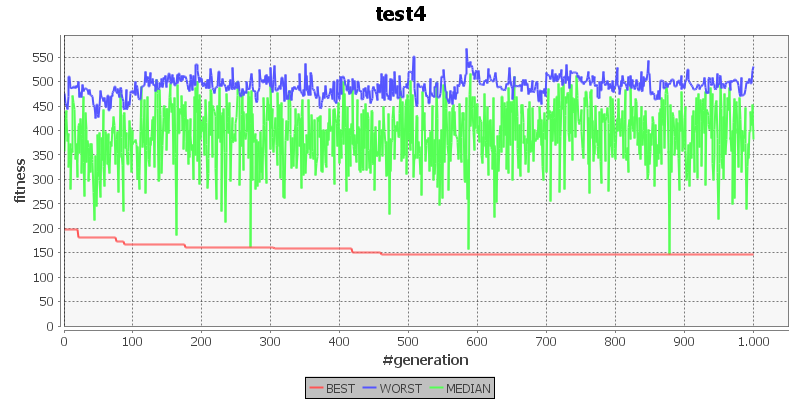
\includegraphics[width=\textwidth]{RouletteSelector.png}
  \caption{RouletteSelector}
\end{minipage}%
\begin{minipage}{.5\textwidth}
  \centering
  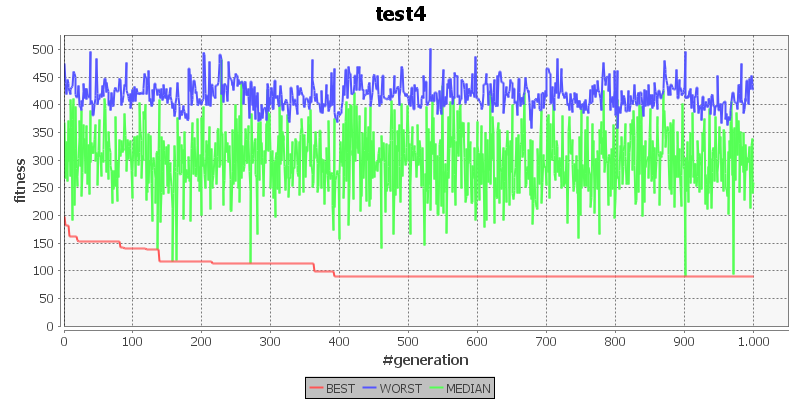
\includegraphics[width=\textwidth]{RandomSelector.png}
  \caption{RandomSelector}
\end{minipage}
\end{figure}

\subsubsection{Cruce: OrderOXCrossover vs. OrderPMXCrossover}

El resto de parámetros se fijo a:

\begin{itemize}[noitemsep]
	\item Selección: \lstinline|RouletteSelector|.
	\item Mutación: \lstinline|Order2OptMutator|.	
\end{itemize}

En la siguiente tabla se muestran los fitness obtenidos para cada uno de los test junto con el instante en el que se realizó el último aterrizaje:
 
\begin{table}[!ht]
\centering
\begin{tabular}{@{}lllll@{}}
\toprule
Algoritmo         & Mejor & Peor & Medio & Último aterrizaje \\ \midrule
OrderOXCrossover  & 137   & 487  & 290   & 17                \\
OrderPMXCrossover & 147   & 531  & 382   & 16                \\ \bottomrule
\end{tabular}
\caption{OrderOXCrossover vs. OrderPMXCrossover}
\end{table}

Los gráficos de la ejecución fueron:

\begin{figure}[!ht]
\centering
\begin{minipage}{.5\textwidth}
  \centering
  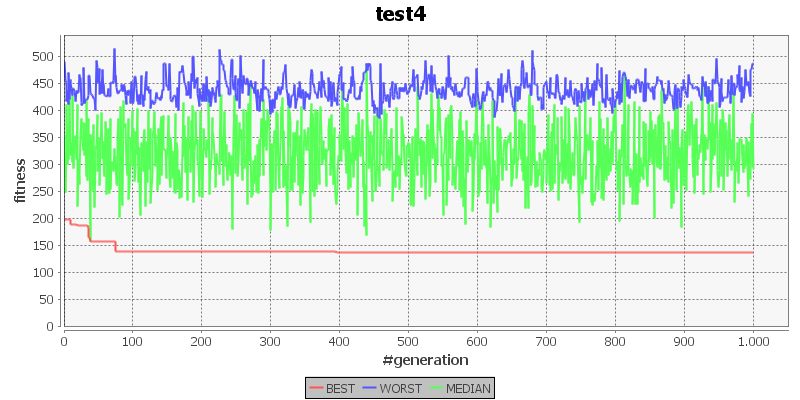
\includegraphics[width=\textwidth]{OrderOXCrossover.png}
  \caption{OrderOXCrossover}
\end{minipage}%
\begin{minipage}{.5\textwidth}
  \centering
  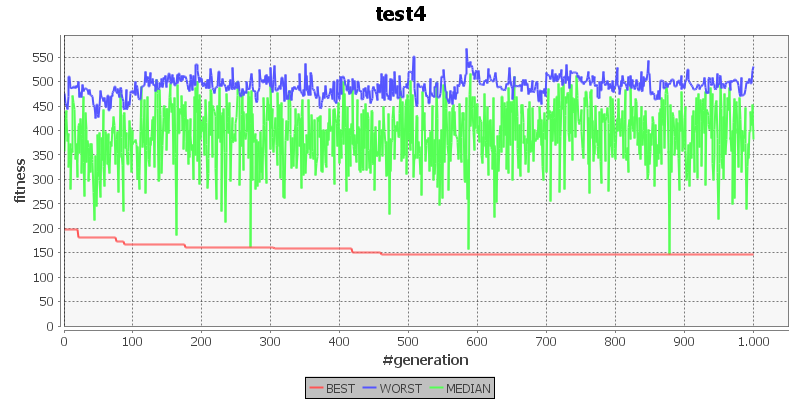
\includegraphics[width=\textwidth]{OrderPMXCrossover.png}
  \caption{OrderPMXCrossover}
\end{minipage}
\end{figure}

\newpage

\subsubsection{Mutación: Order2OptMutator vs. OrderSublistMutator}

El resto de parámetros se fijo a:

\begin{itemize}[noitemsep]
	\item Selección: \lstinline|RouletteSelector|.
	\item Cruce: \lstinline|OrderPMXCrossover|.
\end{itemize}

En la siguiente tabla se muestran los fitness obtenidos para cada uno de los test junto con el instante en el que se realizó el último aterrizaje:

\begin{table}[!ht]
\centering
\begin{tabular}{@{}lllll@{}}
\toprule
Algoritmo           & Mejor & Peor & Medio & Último aterrizaje \\ \midrule
Order2OptMutator    & 147   & 531  & 382   & 16                \\
OrderSublistMutator & 150   & 487  & 388   & 17                \\ \bottomrule
\end{tabular}
\caption{Order2OptMutator vs. OrderSublistMutator}
\end{table}

Los gráficos de la ejecución fueron:

\begin{figure}[!ht]
\centering
\begin{minipage}{.5\textwidth}
  \centering
  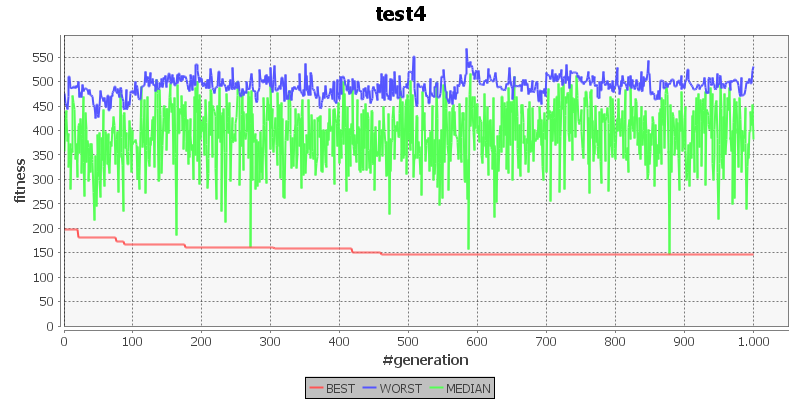
\includegraphics[width=\textwidth]{Order2OptMutator.png}
  \caption{Order2OptMutator}
\end{minipage}%
\begin{minipage}{.5\textwidth}
  \centering
  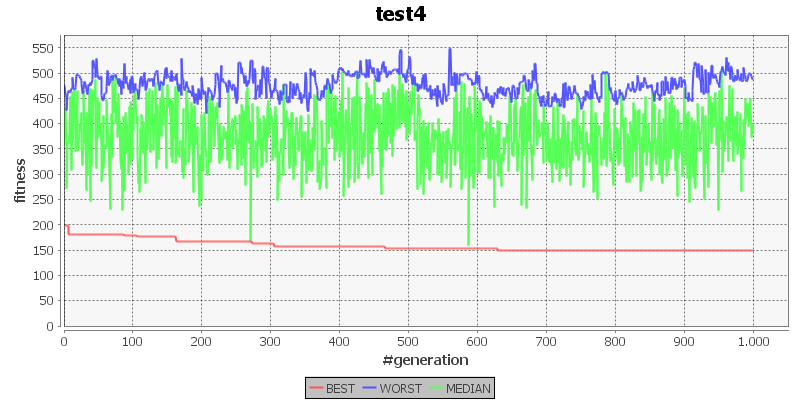
\includegraphics[width=\textwidth]{OrderSublistMutator.png}
  \caption{OrderSublistMutator}
\end{minipage}
\end{figure}

\subsection{Resultados con variación de los parámetros}

A continuación se exponen los resultados de variar ciertos parámetros numéticos del algoritmo. El archivo de pruebas utilizado fue \lstinline|IncomingFlights_4|. Las implementaciones de los operadores genéticos fueron:

\begin{itemize}[noitemsep]
	\item Selección: \lstinline|RouletteSelector|.
	\item Cruce: \lstinline|OrderPMXCrossover|.
	\item Mutación: \lstinline|Order2OptMutator|.	
\end{itemize}

\newpage
\subsubsection{Tamaño de la población}

\begin{table}[!ht]
\centering
\begin{tabular}{@{}lllll@{}}
\toprule
Tamaño & Mejor & Peor & Medio & Último aterrizaje \\ \midrule
50     & 158   & 465  & 327   & 16                \\
500    & 112   & 557  & 508   & 15                \\ \bottomrule
\end{tabular}
\caption{50 vs. 500}
\end{table}

\begin{figure}[!ht]
\centering
\begin{minipage}{.5\textwidth}
  \centering
  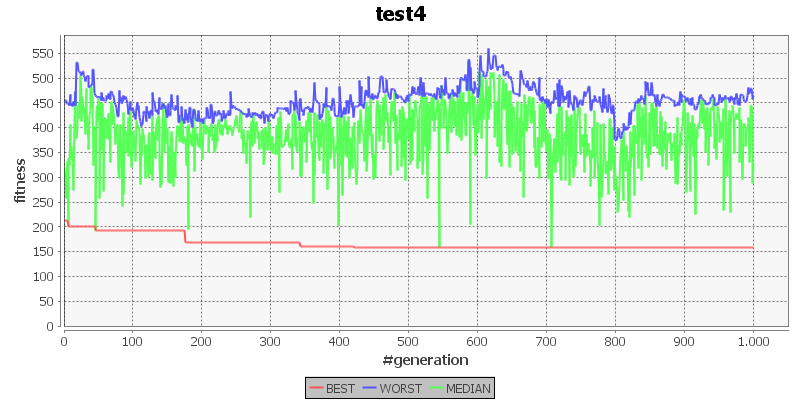
\includegraphics[width=\textwidth]{50tam.png}
  \caption{50}
\end{minipage}%
\begin{minipage}{.5\textwidth}
  \centering
  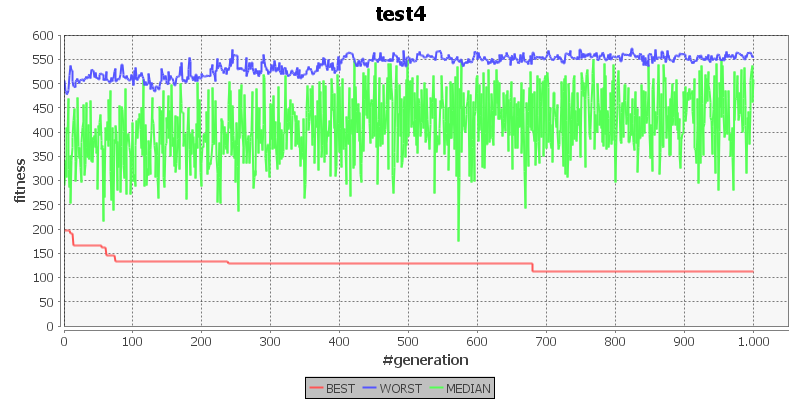
\includegraphics[width=\textwidth]{500tam.png}
  \caption{500}
\end{minipage}
\end{figure}

\subsubsection{Probabilidad de cruce}

\begin{table}[!ht]
\centering
\begin{tabular}{@{}lllll@{}}
\toprule
Probabilidad & Mejor & Peor & Medio & Último aterrizaje \\ \midrule
50\%         & 135   & 529  & 440   & 15                \\
90\%         & 128   & 429  & 389   & 17                \\ \bottomrule
\end{tabular}
\caption{50\% vs. 90\%}
\end{table}

\begin{figure}[!ht]
\centering
\begin{minipage}{.5\textwidth}
  \centering
  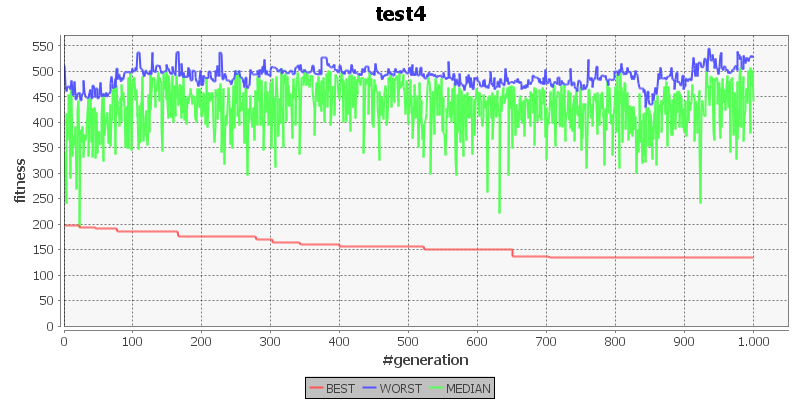
\includegraphics[width=\textwidth]{50cruce.png}
  \caption{50\%}
\end{minipage}%
\begin{minipage}{.5\textwidth}
  \centering
  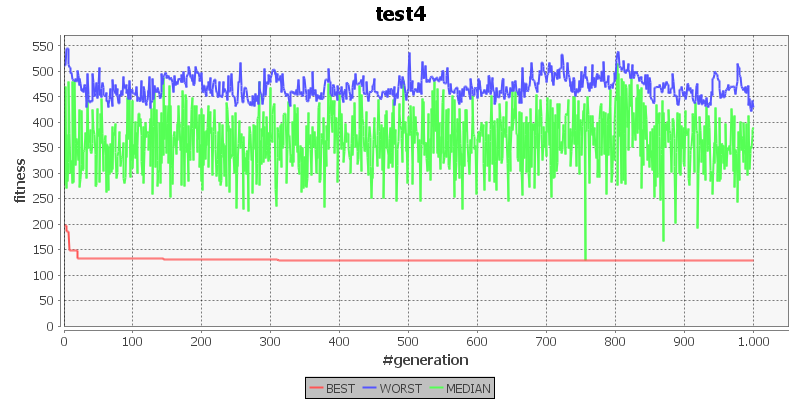
\includegraphics[width=\textwidth]{90cruce.png}
  \caption{90\%}
\end{minipage}
\end{figure}

\newpage

\subsubsection{Probabilidad de mutación}

\begin{table}[!ht]
\centering
\begin{tabular}{@{}lllll@{}}
\toprule
Probabilidad & Mejor & Peor & Medio & Último aterrizaje \\ \midrule
5\%          & 118   & 473  & 409   & 18                \\
20\%         & 126   & 488  & 308   & 17                \\ \bottomrule
\end{tabular}
\caption{5\% vs. 20\%}
\end{table}

\begin{figure}[!ht]
\centering
\begin{minipage}{.5\textwidth}
  \centering
  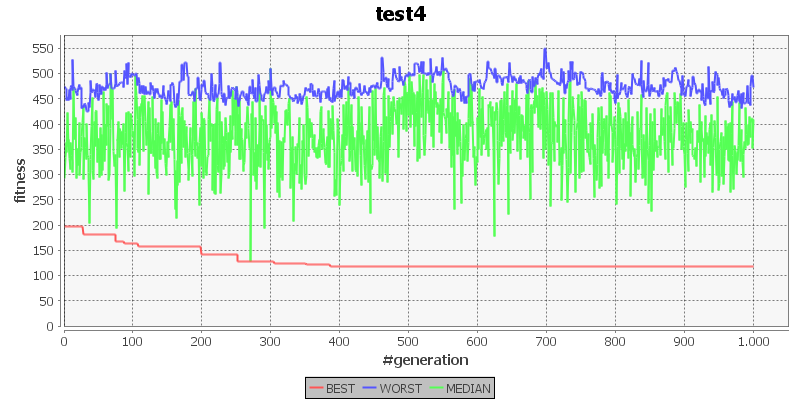
\includegraphics[width=\textwidth]{5mut.png}
  \caption{5\%}
\end{minipage}%
\begin{minipage}{.5\textwidth}
  \centering
  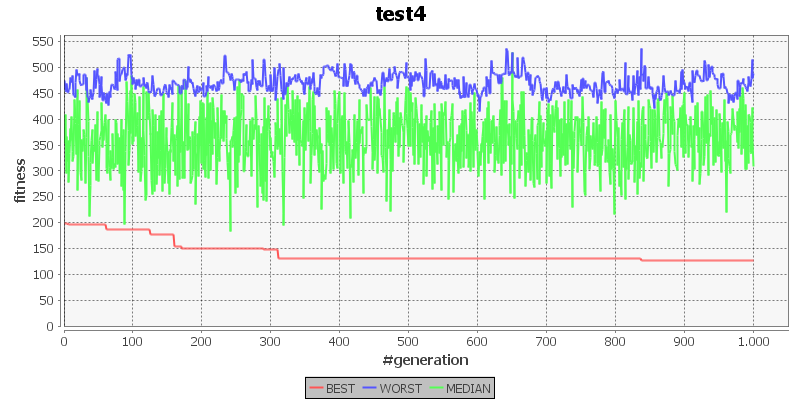
\includegraphics[width=\textwidth]{20mut.png}
  \caption{20\%}
\end{minipage}
\end{figure}

\subsection{Análisis}
Como se ha podido ver a lo largo de toda la sección ha habido algún punto en el que no hemos sido capaces de elegir lo mejor para que el algoritmo fuera capaz de ir mejorando los individuos con las generaciones. 


Principalmente nos parece que el orderarray que usamos puede no ser la mejor opción a la hora del cruce, esto se debe a que dos padres con buena fitness se pueden producir dos individuos no tan buenos.

Por ejemplo, si se hubiesen cruzado los siguientes individuos
genotype = (5 10 17 16 11 19 20 13 14 22 18 7 9 4 1 3 12 21 8 6 2 15 0 23), fitness =[value=222.0]
genotype = (16 22 19 8 10 12 2 4 1 9 5 3 7 0 11 14 6 15 20 21 17 13 18 23), fitness =[value=237.0]

El resultado podría haber sido perfectamente el siguiente (Es un cruce real pero no se sabe si se dio en las pruebas):
(8 10 17 16 11 19 20 13 14 22 18 12 2 4 1 9 5 3 7 0 6 15 21 23), fitness = 216
(17 22 19 8 10 12 2 4 1 9 5 16 11 20 13 14 18 7 3 21 6 15 0 23), fitness = 251

Como podemos ver es cierto que ha mejorado la fitness de uno de los individuos respecto a la del mejor padre, pero tambien es cierto que la de el otro hijo a empeorado bastante. Tambien podemos ver que la media a empeorado desde 229.5 hasta 233.5.

Otro motivo que creemos puede estar influenciando los resultados es que el espacio de busqueda es enorme y debido a nuestra representación no obtienes ninguna informacion de vecinos que estan muy proximos por lo que hace que le sea imposible dar resultados estables.

También nos hemos encontrado con otro problema a la hora de realizar la practica: la dificultad de repetir un buen número de veces cada experimento para obtener resultados fiables en los que los rng no sean la principal causa de un resultado más o menos exitoso.

Una vez habiendo comentado el porque de la forma de la gráfica y los problemas para encontrar resultados validos a nivel científico, vamos a comentar los resultados de las comparaciones de algoritmos que hemos comentado antes y que se nos pide:
 * Selector: Ruleta y Aleatorio
         En este caso podemos atribuir que el aleatorio funcione generalmente mejor que el ruleta por lo que hemos comentado, al reorganizar los numeros lo suficiente para que los hijos no se parezcan en nada a los padres hace que la aleatoriedad pueda ser mucho mejor o mucho peor que la ruleta.

 * Cruce: Order (X)crossover operator  y Partially Matched (X)crossover
         Podemos ver que OX da ligeramente mejores resultados que PMX pero son tan poco mejores que no podemos decir que sean significativos. Otra cosa a tener en cuenta es que PMX explora más de manera que produce más picos tanto hacia los mínimos como hacia los máximos de manera que vemos que esta explorando, esto ultimo puede ser lo que haga que haya encontrado un mínimo mejor.

 * Mutación: 2 Opt y Sublist
         2Opt parece dar mejores resultados y parece que tiene sentido que un algorimo de mutación simple pero potente como 2Opt vaya a dar mejores resultados que Sublist, ya que al modificar menos elementos consigue un punto muy diferente del espacio de busqueda pero con una fitness suficientemente parecida como para que pueda llegar a reproducirse con más probabilidad que Sublist que puede ser que cambie mucho más el elemento y deje la fitness siendo muy mala para cruzarse consistentemente.
	 
En cuanto a la selección de parametros:
 * Tamaño de la población:
         El parametro de tamaño de la población se comporta como esperabamos, cuanta más mejores resultados encuentra por pura fuerza bruta, pero cuando tenemos menos individuos la media es mejor.
	 
 * Probabilidad de cruce:
	 El comportamiento al reducir este parametro es una exploración más lenta del espacio de busqueda, en nuestro ejemplo específico acaba encontrando resultados mejores pero creemos que es por pura coincidencia, aunque podría ser que los optimos esten fuera de la región de optimos locales donde la mayoria de ejecuciones se quedan.
	 
 * Probabilidad de mutacion:
	 Según más aumentemos este parametro más espacios alejados de los optimos actuales exploraremos y que con más probabilidad haya encontrado mejores resultados nos hace sospechar que las mejores soluciones están lejos de algun grupo de optimos locales.
	 
	 
\section{Conclusiones}
El uso de jclec es complejo si se quiere hacer correctamente, no por la complejidad de la biblioteca si no por los problemas que da, por ejemplo cuando genera order array automaticamente tiene un bug y la ultima posicion de dicho array acaba valiendo siempre la longitud del array menos uno. Esto es solo uno de los muchos problemas que tiene como el hecho de que orderarray no este en el paquete principal y este en tutorial. 

Este conjunto de pequeños fallos se van acumulando formando una montaña que dificulta el hecho de usar jclec de manera cientifica o al menos lo más cientifica posible.

Como ultimo cabe destacar el hecho de que existe gran varianza en los resultados obtenidos por el bajo numero de ejecuciones de los mismos, esto no se hubiera dado así si jclec tubiese una manera de reducir varianza, por ejemplo dejando ejecutar el experimento n veces. Consideramos que el framework no esta mal pero parece como si varias personas hubieran hecho distintos proyectos y los hubieran juntado en un momento dado en vez de trabajar conjuntamente.


% -------------------------------------------------------------
% Bibliography
% -------------------------------------------------------------
\newpage
\bibliography{citations}
\bibliographystyle{plainnat}

\end{document}
